\ifx\wholebook\relax \else

\documentclass[UTF8]{article}

%
% loading packages
%

\RequirePackage{ifpdf}
\RequirePackage{ifxetex}

%
%
\ifpdf
  \RequirePackage[pdftex,%
       bookmarksnumbered,%
              colorlinks,%
          linkcolor=blue,%
              hyperindex,%
        plainpages=false,%
       pdfstartview=FitH]{hyperref}
\else\ifxetex
  \RequirePackage[bookmarksnumbered,%
               colorlinks,%
           linkcolor=blue,%
               hyperindex,%
         plainpages=false,%
        pdfstartview=FitH]{hyperref}
\else
  \RequirePackage[dvipdfm,%
        bookmarksnumbered,%
               colorlinks,%
           linkcolor=blue,%
               hyperindex,%
         plainpages=false,%
        pdfstartview=FitH]{hyperref}
\fi\fi
%\usepackage{hyperref}

% other packages
%--------------------------------------------------------------------------
\usepackage{graphicx, color}
\usepackage{wrapfig}
\usepackage{subfig}
\usepackage{multicol}
\usepackage{tikz}
\usetikzlibrary{matrix,positioning,shapes}
\usetikzlibrary{patterns}

\usepackage{amsmath, amsthm, amssymb} % for math
\usepackage{exercise} % for exercise
\usepackage{import} % for nested input

%
% for programming
%
\usepackage{verbatim}
\usepackage{fancyvrb}
\usepackage{listings}
%\usepackage{algorithmic} %old version; we can use algorithmicx instead
%\usepackage[plain]{algorithm} %remove rule (horizontal line on top/below the algorithm
\usepackage{algorithm} %to remove rules change to \usepackage[plain]{algorithm}
%\usepackage{algorithm2e}
\usepackage[noend]{algpseudocode} %for pseudo code, include algorithmicsx automatically
\usepackage{appendix}
\usepackage{makeidx} % for index support
\usepackage{titlesec}
\usepackage{epigraph}

\usepackage[cm-default]{fontspec}
\usepackage{xunicode}
%\usepackage{fontenc}
\usepackage{textcomp}
\usepackage{url}

% detect and select Chinese font
% ------------------------------
% fc-list :lang=zh    % list all Chinese fonts
% fc-list :mono       % list all mono fonts
% fc-cache            % refresh cache to load new installed fonts
\def\macmainfont{STSong}  % Under Mac OS X
\def\macmonofont{Monaco}
\def\winmainfont{SimSun} % Under Windows
\def\winmonofont{Consolas}
\def\linuxmainfont{WenQuanYi Micro Hei} % Under Linux
\def\linuxmainfont{Courier}

\suppressfontnotfounderror1 % Avoid setting exit code (error level) to break make process
\count255=\interactionmode
\batchmode

% main font
\let\mainft=\macmainfont
\font\thefont="\mainft"\space at 10pt
\ifx\thefont\nullfont
  \let\mainft=\winmainfont
  \font\thefont="\mainft"\space at 10pt
  \ifx\the\nullfont
    \let\mainft=\linuxmainfont
    \font\thefont="\mainft"\space at 10pt
    \ifx\the\nullfont
      \errorstopmode
      \errmessage{no suitable Chinese main font found}
    \fi
  \fi
\fi

% mono font
\let\monoft=\macmonofont
\font\thefont="\monoft"\space at 10pt
\ifx\thefont\nullfont
  \let\monoft=\winmonofont
  \font\thefont="\monoft"\space at 10pt
  \ifx\the\nullfont
    \let\monoft=\linuxmonofont
    \font\thefont="\monoft"\space at 10pt
    \ifx\the\nullfont
      \errorstopmode
      \errmessage{no suitable mono font found}
    \fi
  \fi
\fi

\interactionmode=\count255

\setmainfont[Mapping=tex-text]{\mainft}
\setmonofont[Scale=MatchLowercase]{\monoft}   % 英文等宽字体

\XeTeXlinebreaklocale "zh"  % to solve the line breaking issue
\XeTeXlinebreakskip = 0pt plus 1pt minus 0.1pt

\titleformat{\paragraph}
{\normalfont\normalsize\bfseries}{\theparagraph}{1em}{}
\titlespacing*{\paragraph}
{0pt}{3.25ex plus 1ex minus .2ex}{1.5ex plus .2ex}

\lstdefinelanguage{Smalltalk}{
  morekeywords={self,super,true,false,nil,thisContext}, % This is overkill
  morestring=[d]',
  morecomment=[s]{"}{"},
  alsoletter={\#:},
  escapechar={!},
  literate=
    {BANG}{!}1
    {UNDERSCORE}{\_}1
    {\\st}{Smalltalk}9 % convenience -- in case \st occurs in code
    % {'}{{\textquotesingle}}1 % replaced by upquote=true in \lstset
    {_}{{$\leftarrow$}}1
    {>>>}{{\sep}}1
    {^}{{$\uparrow$}}1
    {~}{{$\sim$}}1
    {-}{{\sf -\hspace{-0.13em}-}}1  % the goal is to make - the same width as +
    %{+}{\raisebox{0.08ex}{+}}1		% and to raise + off the baseline to match -
    {-->}{{\quad$\longrightarrow$\quad}}3
	, % Don't forget the comma at the end!
  tabsize=2
}[keywords,comments,strings]

% for literate Haskell code
\lstdefinestyle{Haskell}{
  flexiblecolumns=false,
  basewidth={0.5em,0.45em},
  morecomment=[l]--,
  literate={+}{{$+$}}1 {/}{{$/$}}1 {*}{{$*$}}1 {=}{{$=$}}1
           {>}{{$>$}}1 {<}{{$<$}}1 {\\}{{$\lambda$}}1
           {\\\\}{{\char`\\\char`\\}}1
           {->}{{$\rightarrow$}}2 {>=}{{$\geq$}}2 {<-}{{$\leftarrow$}}2
           {<=}{{$\leq$}}2 {=>}{{$\Rightarrow$}}2
           {\ .}{{$\circ$}}2 {\ .\ }{{$\circ$}}2
           {>>}{{>>}}2 {>>=}{{>>=}}2
           {|}{{$\mid$}}1
}

% "define" Scala
\lstdefinelanguage{Scala}{
  morekeywords={abstract,case,catch,class,def,%
    do,else,extends,false,final,finally,%
    for,if,implicit,import,match,mixin,%
    new,null,object,override,package,%
    private,protected,requires,return,sealed,%
    super,this,throw,trait,true,try,%
    type,val,var,while,with,yield},
  otherkeywords={=>,<-,<\%,<:,>:,\#,@},
  sensitive=true,
  morecomment=[l]{//},
  morecomment=[n]{/*}{*/},
  morestring=[b]",
  morestring=[b]',
  morestring=[b]"""
}

\lstloadlanguages{C, C++, Java, Lisp, Haskell, Python, Smalltalk, Scala}

\lstset{
  basicstyle=\small\ttfamily,
  commentstyle=\rmfamily,
  texcl=true,
  showstringspaces = false,
  upquote=true,
  flexiblecolumns=false
}

\newcommand\doubleplus{+\kern-1.3ex+\kern0.8ex}

% ======================================================================

\def\BibTeX{{\rm B\kern-.05em{\sc i\kern-.025em b}\kern-.08em
    T\kern-.1667em\lower.7ex\hbox{E}\kern-.125emX}}

%
% mathematics
%
\newcommand{\be}{\begin{equation}}
\newcommand{\ee}{\end{equation}}
\newcommand{\bmat}[1]{\left( \begin{array}{#1} }
\newcommand{\emat}{\end{array} \right) }
\newcommand{\VEC}[1]{\mbox{\boldmath $#1$}}

% numbered equation array
\newcommand{\bea}{\begin{eqnarray}}
\newcommand{\eea}{\end{eqnarray}}

% equation array not numbered
\newcommand{\bean}{\begin{eqnarray*}}
\newcommand{\eean}{\end{eqnarray*}}

\newtheorem{theorem}{定理}[section]
\newtheorem{lemma}[theorem]{引理}
\newtheorem{proposition}[theorem]{Proposition}
\newtheorem{corollary}[theorem]{Corollary}

% 中文书籍设置
% ====================================
\renewcommand\contentsname{目\ 录}
%\renewcommand\listfigurename{插图目录}
%\renewcommand\listtablename{表格目录}
\renewcommand\figurename{图}
\renewcommand\tablename{表}
\renewcommand\proofname{证明}
\renewcommand\ExerciseName{练习}
%\renewcommand{\algorithmcfname}{算法}

\ifx\wholebook\relax
\renewcommand\bibname{参\ 考\ 文\ 献}                    %book类型
%\newtheorem{Definition}[Theorem]{定义}
\newtheorem{Theorem}{定理}[chapter]
\newtheorem{example}{例题}[chapter]
\else
\renewcommand\refname{参\ 考\ 文\ 献}
\fi

%\setcounter{secnumdepth}{4}
\titleformat{\chapter}
  {\normalfont\bfseries\Large}
  {第\arabic{chapter}章}
  {12pt}{\Large}
%% \titleformat{\subsection}
%%   {\normalfont\bfseries\large}
%%   {\CJKnumber{\arabic{subsection}}、}
%%   {12pt}{\large}
%% \titleformat{\subsubsection}
%%   {\normalfont\bfseries\normalsize}
%%   {\arabic{subsubsection}.}
%%   {12pt}{\normalsize}

%\renewcommand{\baselinestretch}{1.5}                        %文章行间距为1.5倍。

\makeatletter
\newcommand{\verbatimfont}[1]{\renewcommand{\verbatim@font}{\ttfamily#1}}
\makeatother

\setcounter{tocdepth}{4}
\setcounter{secnumdepth}{4}

%\verbatimfont{\footnotesize}


\setcounter{page}{1}

\begin{document}

\title{递归}

\author{刘新宇
\thanks{{\bfseries 刘新宇} \newline
  Email: liuxinyu95@gmail.com \newline}
  }

\maketitle
\fi

\markboth{递归}{编程的数学原理}

\epigraph{\textbf{造物神}是\textbf{造}物主\textbf{物}色的\textbf{神}怪}{——[美]侯世达《哥德尔、埃舍尔、巴赫——集异壁之大成》}

\section{万物皆数}

\begin{wrapfigure}{R}{0.3\textwidth}
%\begin{figure}[htbp]
 \centering
 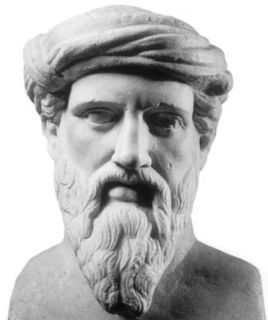
\includegraphics[scale=0.4]{img/Pythagoras.eps}
 \captionsetup{labelformat=empty}
 \caption{毕达哥拉斯(约前570——前490)}
 \label{fig:Pythagoras}
%\end{figure}
\end{wrapfigure}

人们通过深入了解数进而了解自然。在上一章中,我们介绍了自然数的皮亚诺公理。并且展示了一些和自然数有着相同结构的事物,包括计算机系统中的基本数据结构列表。自然数成为了我们进一步前进的基石。但是我们的大厦还不稳固。第一章中,我们不加证明地使用了递归的概念。例如阶乘的定义:

\[
\begin{array}{l}
fact(0) = 1 \\
fact(n + 1) = (n + 1) \cdot fact(n)
\end{array}
\]

以及$foldn$的实现:

\[
\begin{array}{l}
foldn(z, f, 0) = z \\
foldn(z, f, n') = f(foldn(z, f, n))
\end{array}
\label{eq:foldn}
\]

递归的原理是什么?为什么它是正确的?递归可以在更低的层次被表示么?这些都是我们在这一章要解决的问题。

毕达哥拉斯的介绍,万物皆数的哲学思想(三角形数,音乐)。公度的概念,无理数的发现和递归的关系。


%\begin{wrapfigure}{R}{0.5\textwidth}
%% \begin{figure}[htbp]
%%  \centering
%%  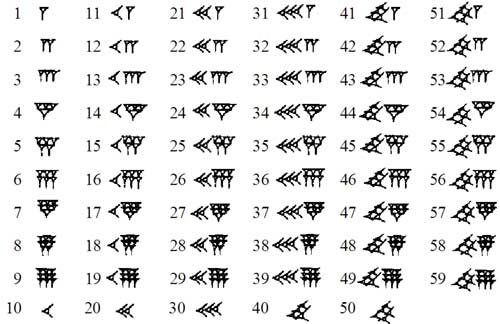
\includegraphics[scale=0.6]{img/Babylonian_numerals.eps}
%%  \caption{巴比伦楔形文字中的数字\cite{wiki-babylonian-num}。}
%%  \label{fig:babylonian-num}
%% \end{figure}
%\end{wrapfigure}

%\begin{wrapfigure}{R}{0.5\textwidth}
%% \begin{figure}[htbp]
%%  \centering
%%  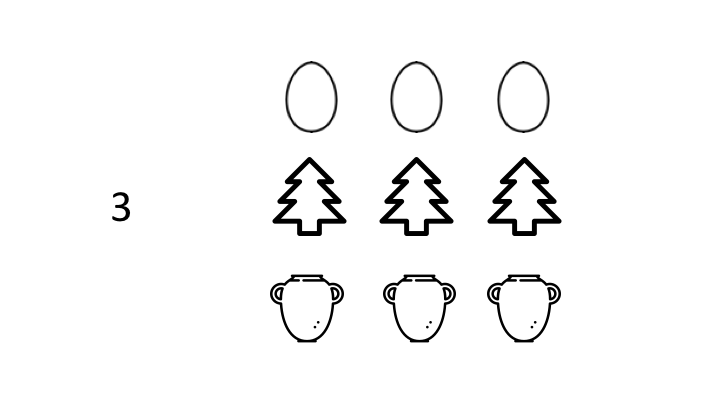
\includegraphics[scale=0.2]{img/abstract-num.eps}
%%  \caption{具体的三个事物和抽象的数字三}
%%  \label{fig:abstract-num}
%% \end{figure}
%\end{wrapfigure}

\section{欧几里得算法}

%\begin{wrapfigure}{R}{0.4\textwidth}
%% \begin{figure}[htbp]
%%  \centering
%%  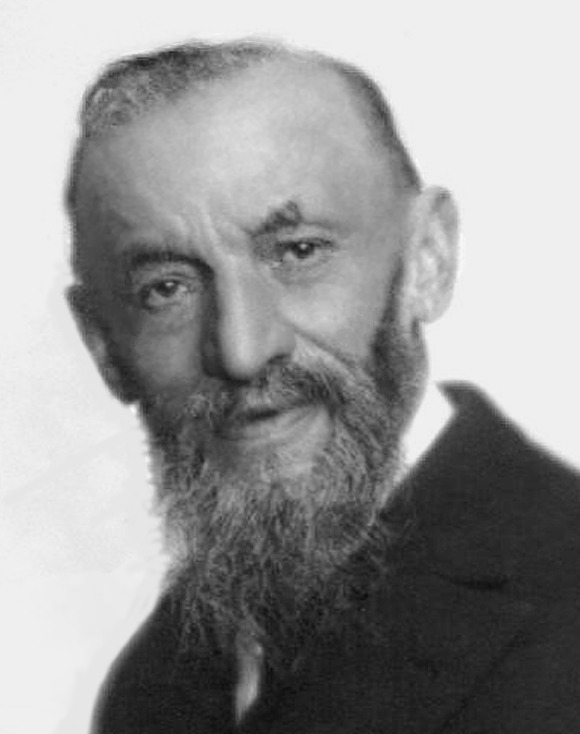
\includegraphics[scale=0.2]{img/Peano.eps}
%%  \caption{朱塞佩$\cdot$皮亚诺(Giuseppe Peano)1858 - 1932。}
%%  \label{fig:Peano}
%% \end{figure}
%\end{wrapfigure}

欧几里得最大公约数(公度)算法的概念。几何量和数的分离。最大公约数算法的意义,递归原理问题的提出

扩展欧几里得算法、倒水趣题。

\section{$\lambda$演算}

lambda的由来,三大变换:Alpha, Beta, Eta变换,变换与归约。

%\begin{figure}[htbp]
\begin{wrapfigure}{R}{0.4\textwidth}
\centering
\begin{tikzpicture}[scale=0.8]
\filldraw[fill=gray, draw=black, pattern=north west lines] (0, 0) rectangle (2, 1)
    (2, 0) rectangle (3, 1);
\draw (3, 0) rectangle (4.5, 1);
\draw (0, -1) rectangle (2, -2);
\filldraw[fill=gray, draw=black, pattern=north west lines] (2, -1) rectangle (3, -2)
    (3, -1) rectangle (4.5, -2);
\end{tikzpicture}
\caption{加法结合律的几何证明。上下面积相等}
\end{wrapfigure}
%\end{figure}

%\begin{wrapfigure}{R}{0.4\textwidth}
\begin{figure}[htbp]
\centering
\begin{tikzpicture}[scale=0.8]
\draw (0, 0) rectangle (2, 1)
    (2, 0) rectangle (3, 1);
\draw (0, -1) rectangle (1, -2)
    (1, -1) rectangle (3, -2);
\end{tikzpicture}
\caption{加法交换律的几何证明。将上方的图形倒过来看,或者在镜中看。}
\end{figure}
%\end{wrapfigure}

\begin{Exercise}
\begin{enumerate}
\item 一些lambda演算的练习
\end{enumerate}
\end{Exercise}

\section{递归的定义}

Y组合子和递归的定义
%% \begin{wrapfigure}{R}{0.4\textwidth}
%% %\begin{figure}[htbp]
%%  \centering
%%  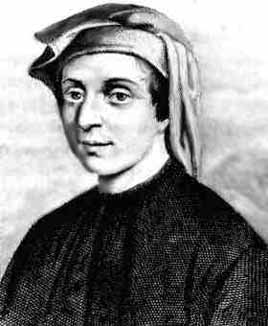
\includegraphics[scale=0.4]{img/Fibonacci.eps}
%%  \caption{比萨的列奥纳多,又称斐波那契(Leonardo Pisano, Fibonacci),1175年-1250年}
%%  \label{fig:Fibonacci}
%% %\end{figure}
%% \end{wrapfigure}


%\begin{wrapfigure}{L}{0.3\textwidth}
%% \begin{figure}[htbp]
%%  \centering
%%  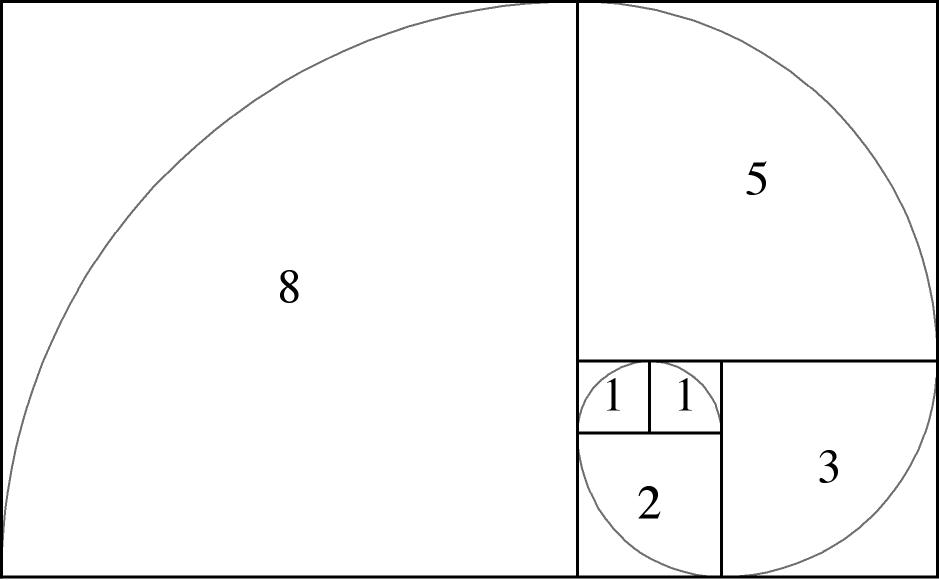
\includegraphics[scale=0.5]{img/fibonacci_spiral.eps}
%%  \caption{这些正方形的边长组成了斐波那契序列。}
%%  \label{fig:fibonacci_spiral}
%% \end{figure}
%\end{wrapfigure}

%\begin{wrapfigure}{R}{0.3\textwidth}
%% \begin{figure}[htbp]
%%  \centering
%%  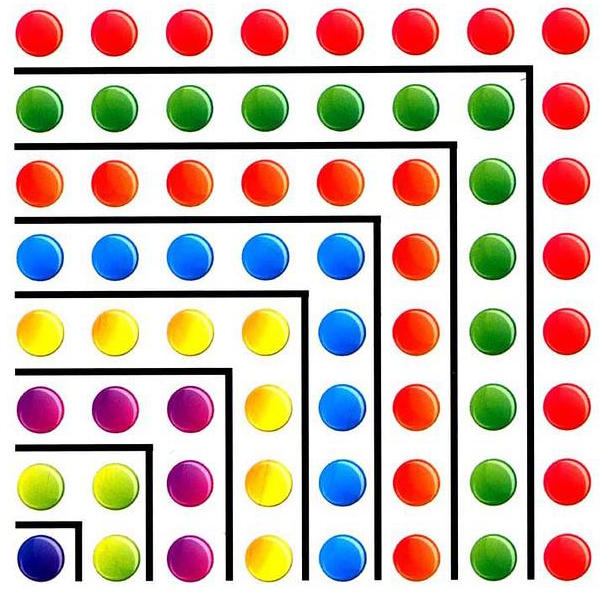
\includegraphics[scale=0.2]{img/PWW.eps}
%%  \caption{《无需语言的证明》封面局部}
%%  \label{fig:PWW}
%% \end{figure}
%\end{wrapfigure}

\section{$\lambda$的意义}

CONS/HEAD/TAIL的lambda表示。

二叉树、多叉树的递归结构与FOLD

\section{递归的结构与形式}

%\begin{wrapfigure}{R}{0.3\textwidth}
%% \begin{figure}[htbp]
%%  \centering
%%  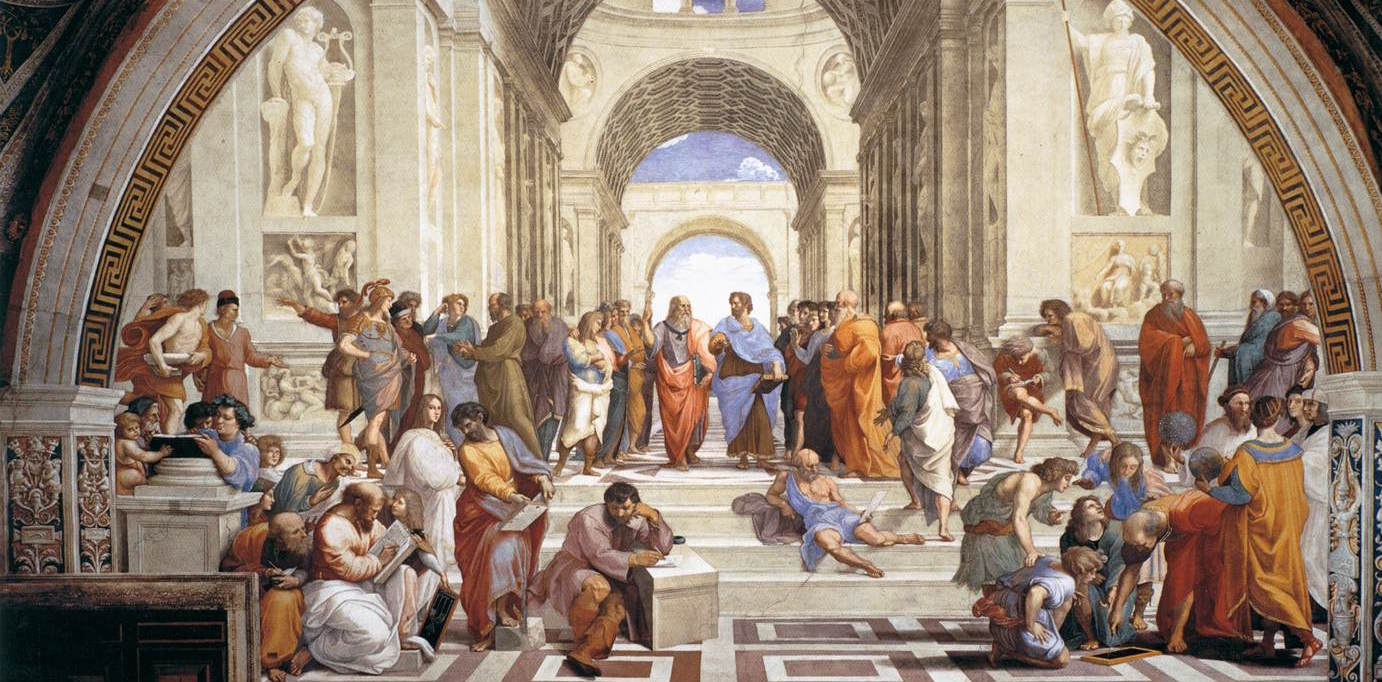
\includegraphics[scale=1.0]{img/the-school-of-athens.eps}
%%  \caption{拉斐尔《雅典学院》局部}
%%  \label{fig:the-school-of-athens}
%% \end{figure}
%\end{wrapfigure}

递归的形式之美——分形与艺术

递归的结构之美——文艺和音乐作品

\ifx\wholebook\relax \else
\begin{thebibliography}{99}

\bibitem{wiki-number}
Wikipedia. ``古代计数系统的历史''. \url{https://en.wikipedia.org/wiki/History_of_ancient_numeral_systems}

\bibitem{trip-to-number-kindom}
[美]卡尔文$\cdot$C$\cdot$克劳森. ``数学旅行家:漫游数王国''. 袁向东、袁钧译,上海教育出版社。ISBN: 7-5320-7883-3/G $cdot$ 7972

\bibitem{wiki-babylonian-num}
Wikipedia. ``古巴比伦数字''. \url{https://en.wikipedia.org/wiki/Babylonian_numerals}

\bibitem{GEB}
[美]候世达 ``哥德尔、埃舍尔、巴赫——集异壁之大成''. 商务印书馆 1996. ISBN: 978-7-100-01323-9

\bibitem{Bird97}
Richard Bird, Oege de Moor. ``Algebra of Programming''. University of Oxford, Prentice Hall Europe. 1997. ISBN: 0-13-507245-X.

\bibitem{Gusen2014}
顾森 ``浴缸里的惊叹''. 人民邮电出版社. 2014, ISBN: 9787115355744

\end{thebibliography}

\expandafter\enddocument
%\end{document}

\fi
